\chapter{Development Process and Tools}\label{devProcChap}
This chapter, after having introduced the agile development framework \emph{Scrum}, describes the development process adopted by the team in order to complete the work.

	%TODO: qui i corsivi sono usati quando il termine è usato per la prima volta senza essere stato definito (non è una convenzione)
	\section{Scrum}\label{ref_scrum}
	\emph{Scrum} is a framework for the agile management of the project development. 
	As such, it does not define the technical way in which the developers must do the job but it follows the development process. 	
	The framework has many dimensions: roles, events, rules and artifacts within the framework serve specific purposes and contribute the Scrum's success~\cite{scrumEnglishGuide}.  

	The following sections describe one by one these components. The first section describes the main roles of people within the framework, the second focuses on the events and the meetings necessary for the implementation of the methodology and the third one puts in evidence the artifacts needed.

	All the information about Scrum are taken from~\cite{scrumEnglishGuide}. See it for a more detailed description.

	\begin{figure}[h]
	  \begin{center} 
		%immagine senza copywright  :)
	    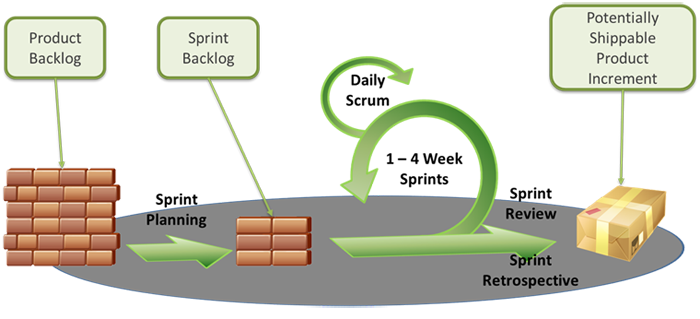
\includegraphics[scale=0.45]{images/ch_04/scrum_overview.png}
	  \end{center} 
	  \caption{\textit{Overview of the Scrum Process}}  
	  \label{fig:ScrumOverview}
  	\end{figure}

\newpage

		\subsection{The Scrum Team}\label{ref_scrum_team}
		The \emph{Scrum Team} is composed of a \emph{Product Owner}, the \emph{Development Team}, and a \emph{Scrum Master}.
		These figures have different roles but all of them have to reach the same goal, add to the product a finite and usable set of new features at constant time intervals. %(see \ref{ref_scrum_sprint_plan}). 

		Scrum Teams are self-organized and cross-functional. Self-organization gives the members the possibility to choose the best way to accomplish their work, without being directed by others outside the team. This fact not only avoids the team to be directed by someone who has not the technical knowledge to solve specific problems and, consequently, can not find the best ways to achieve the goals, but also allows the Team to optimize its own development process. Moreover, the consequent improvement of the sense of ownership that the Team feels on the product increases the motivation of the members. Cross-functionality gives the team all the competencies needed to accomplish the work without depending on others not part of the team. In this way, all the tasks can be accomplished directly by the team, thus the team is never blocked waiting for the work of someone outside it. 


		The delivery of the products is iterative and incremental. This fact guarantees a constant feedback on the correctness of the job and ensures that a deliverable version of the product is always available.

		The following paragraphs will describe each of the three roles.

		\begin{figure}[h]
		  \begin{center} 
			%immagine senza copywright  :)
		    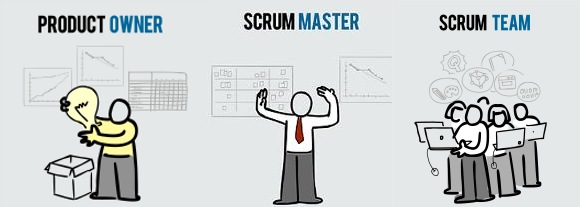
\includegraphics[scale=0.75]{images/ch_04/scrum_team_final.jpg}
		  \end{center} 
		  \caption{\textit{The Scrum Team}}  
		  \label{fig:ScrumTeam}
	  	\end{figure}
			

			\subsubsection{Product Owner}\label{ref_prod_owner}
			The \emph{Product Owner} is the person who represents the stakeholders of the product and is responsible for the performance of the team. His role is to define the requirements for each new version of the product, assign them the priorities and explain them to the team in detail. 
			The requirements are called \emph{Backlog Items} and are included in the \emph{Product Backlog}. This document is described in more details in section \ref{ref_scrum_artifacts}.
			
			Scrum rules require a person to assume the role of Product Owner to represent the will of a committee. 
			In this way, he assumes an intermediation role for all the communications between the developers and the stakeholders and becomes a reference point for both these categories. 
			On one side, he has to give the stakeholders all the information about the progress of the development and the performances of the team. On the other hand, he has to decide the priorities of the tasks and deliver the team the messages of the stakeholders.
			

			\subsubsection{Development Team}\label{ref_scrum_dev_team}
			The \emph{Development Team} consists of professionals programmers, whose role is to implement the new functionalities to the product. The team is usually composed of a number of members which varies from three to nine. 	
			One team must be self-organizing, this means that only the members can decide step by step the tasks in which the items are split and how to accomplish each of them in order to add functionalities to the product. 
			Every team is also cross-functional, i.e. is composed of people who have different skills. In this way it can be autonomous and it does not have to depend on other people outside the team to accomplish its job.
			The more synergy the Development Team has, the higher its overall efficiency and effectiveness are.
 
			\subsubsection{Scrum Master}\label{ref_scrum_master}
			The \emph{Scrum Master} has the role to verify that the Scrum process is understood and put in place. He does this by checking that everyone in the team follows Scrum theory, practices, and rules. 
			The Scrum Master is the enforcer of the rules and interacts with all the people inside and outside the Scrum Team in order to avoid useless interactions.
			On one side, he helps the Product Owner finding techniques for managing the \emph{Product Backlog}, teaching him how to communicate in clear way with the Development Team and understanding and practicing the agile development. On the other hand, he coaches the Development Team in self-organization and cross-functionality, he protects it from unhelpful interruptions and keeps it focused on the tasks. 
			For this, often this role is referred as a \emph{"servant-leader for the Scrum Team"}~\cite[p.6]{scrumEnglishGuide}.


		\subsection{Events}\label{ref_scrum_events}
			Prefixed meetings in Scrum have the purpose of marking time and hence minimizing the need for meetings not defined in Scrum, which can distract the members of the team from their tasks. In this events, different roles in the Scrum Team can interact with regularity, without the need for continuous interruptions. All the events are time-boxed, i.e. every event has a maximum duration. This ensures that only the appropriate amount of time is spent planning, avoiding wasting time. 

			The following sections describe the \emph{Sprint}, the \emph{Sprint Planning Meeting}, the \emph{Daily Scrum}, the \emph{Sprint Review} and the \emph{Sprint Retrospective}.

			\begin{figure}[h]
			  \begin{center} 
				%immagine senza copywright  :)
			    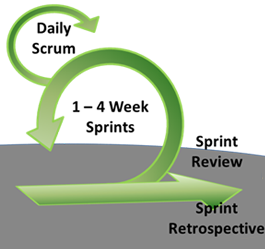
\includegraphics[scale=0.8]{images/ch_04/scrum_events.png}
			  \end{center} 
			  \caption{\textit{The Scrum Events}}  
			  \label{fig:ScrumEvents}
		  	\end{figure}
			


			
			\subsubsection{Sprint}\label{ref_scrum_sprint}
			The \emph{Sprint} is the primary unit of development in Scrum. It is a time-box with a prefixed duration and can last from one week to one month. During this period of time the team creates a self-contained portion of product. 

			Each Sprint starts with the \emph{Sprint Planning Meeting} and ends with the \emph{Sprint Review Meeting} and the \emph{Sprint Retrospective Meeting}. All these events will be described in more detail in the next sections.  
		
\begin{comment}	
			Each Sprint is preceded by a \emph{Sprint Planning Meeting}, where the Scrum Team defines the tasks for the Sprint and gives an estimation for the Sprint Goal. It ends with the \emph{Sprint Review Meeting} and \emph{Sprint Retrospective Meeting}, where the Scrum Team respectively reviews the progress and analyses the mistakes in the Scrum method and proposes solutions in order to avoid it in the next Sprint. All these events will be described with more details in the next sections.  
\end{comment}

			\subsubsection{Sprint Planning Meeting}\label{ref_scrum_sprint_plan}
			The \emph{Sprint Planning Meeting} is a meeting at which all the member of the Scrum Team participate. It is the beginning of every Sprint. In this meeting the team decides the new features the product will include by the end of the Sprint.

			At first the Product Owner informs the team about the features that he wants to be added to the product, each one with its priority. Each one is an item in the \emph{Product Backlog}, which is described in the section \ref{ref_scrum_prod_backlog}. Then, the Development Team estimates how long it would take to add each of the new features to the product and, consequently, how many of them will be added by the end of the Sprint. Often in this part of the meeting the Product Owner and the Development Team have a talk in order to define better the requirements. This fact guarantees that the developed features adhere strictly to the requirements and leads to a new time estimation for most of the goals. 

			The goals are split into tasks, each of which takes no more than two days to be accomplished by the Development Team. Every task and the delivery plan are collected in the \emph{Sprint Backlog}, described in the section \ref{ref_scrum_sprint_backlog}.

			Every Sprint must have a \emph{Sprint Goal}. The Sprint Goal acts like a sort of motivation which reminds the Development Team during the whole Sprint which is in a wider context the goal of their activities. For this reason the Sprint Goal should not be changed during the Sprint.
		
			\subsubsection{Daily Scrum}\label{ref_scrum_daily}
			The \emph{Daily Scrum} is a fifteen minutes event for the Development Team and the Scrum Master, that allows the team to synchronize the work and plan the next day activities. This purpose is achieved analyzing the work done in the last day and forecasting the work for the next one. 
			During the meeting, each Development Team member explains what he did since the last meeting, what he is going to do before the next meeting and the problems he had to front.
			The meeting has the purpose of evaluating the progress towards the Sprint Goal and analyzing the trend of the progress in comparison with the Sprint Backlog. This allows the Scrum Team to measure its speed and, consequently, to make better time estimations in the next Sprints. 

			\subsubsection{Sprint Review}\label{ref_scrum_sprint_rev}
			The \emph{Sprint Review} is a time-boxed meeting which closes every Sprint. In this meeting the increment of the work is analyzed and, if needed, the Product Backlog is updated. 
			During the meeting, the Product Owner analyzes what has been completed and what has not. The Development Team describes the problems it encountered, how it solved them and shows the new functionalities added to the product. Then the whole team discusses of new features to be added, old ones to be deleted or how to improve other ones and, more generally, collaborates on what to do next, updating consequently the Product Backlog.			

			\subsubsection{Sprint Retrospective}\label{ref_scrum_sprint_retro}
			The \emph{Sprint Retrospective} is a time-boxed meeting that takes place after ever Sprint Review. It is an opportunity for the Scrum Team to analyze its Scrum implementation and create a plan to improve the next Sprint. 
			During the meeting the focus is set on people, relationships, processes and tools. The most important successes are shown and a plan for implementing potential improvements is created. 
			The purpose of this meeting is to make the implementation of the Scrum method more effective by optimizing the development process and introducing techniques that make the method more productive and enjoyable. 

		
		\subsection{Artifacts}\label{ref_scrum_artifacts}
			Scrum's \emph{artifacts} represent the work in many different ways. The basic artifacts required by the framework are the \emph{Product Backlog} and the \emph{Sprint Backlog}.

			\subsubsection{Product Backlog}\label{ref_scrum_prod_backlog}
			The \emph{Product Backlog} is an artifact which contains the list of the requirements for a product. The elements of the list, called \emph{Backlog Items}, are sorted by priority.

			Every Item must have a name, a description, an estimate and a priority. For each Item, the Product Owner, representing the stakeholder, sets the priority and the Development Team defines the estimate.

			The Product Backlog is dynamic. Its earliest versions only contain the initially and best understood requirements of the product. Then, as long as the product evolves and new requirements are introduced, it is continuously updated. In this way, it always contains all the features, enhancements and fixes that must be added in the future to the product.  

			As the higher ordered Items are more important than lower ordered ones, they are clearer and more detailed. The team can make more precise estimates thanks to the greater clarity and increased detail. 
%The lower the order of the items, the less detailed are the description and the time estimation.  \todo{correggi questa frase}
			
			The activity of adding detail, estimates and sort the items in the Product Backlog is called \emph{grooming}. The Scrum Team decides how and when to do it. Anyway the grooming activity must not consume more than the 10\% of the capacity of the team. 
		

			\subsubsection{Sprint Backlog}\label{ref_scrum_sprint_backlog}
			The \emph{Sprint Backlog} contains the Product Backlog Items selected for the current Sprint and a plan for completing all the modifications to the product and realizing the Sprint Goal. 
			The Sprint Backlog contains all the functionalities that should be added to the product by the end of the Sprint, each of which with its estimates and priorities, and, at the same time, monitors the state of the work during every day of the Sprint.
			
			\begin{figure}[h]
			  \begin{center} 
			    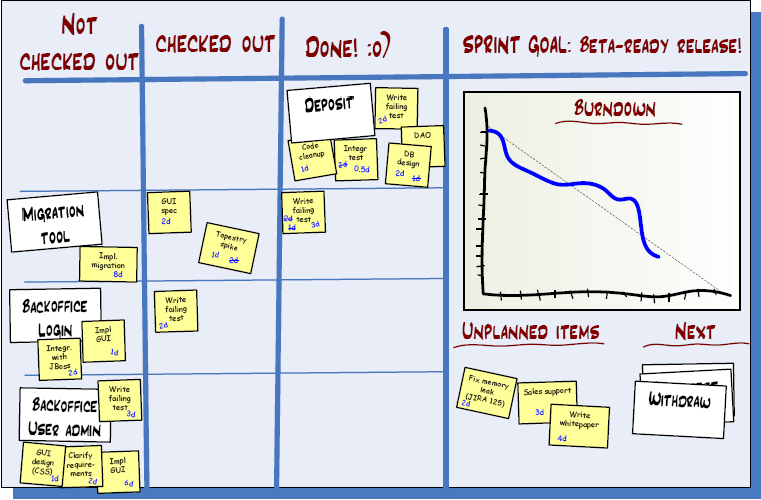
\includegraphics[scale=0.65]{images/ch_04/task_board_and_chart.png}
			  \end{center} 
			  \caption{\textit{Sprint Backlog and Burn Down Chart}}  
			  \label{fig:SprintBacklog}
		  	\end{figure}
\begin{comment}
			The level of detail of the work is such that it can be measured during the Daily Scrum.	The stimate of each task can not be longer than 16 hours.

			The Backlog Items represent such features each of which is split into tasks that must be accomplished in not more than than sixteen hours of work. The tasks are never assigned; rather, each member of the team takes charge of some of them during the Daily Scrum, according to the set priority and his own skills. 
\end{comment}
			The level of detail of the work is such that it can be measured during the Daily Scrum. 
			In this meeting, in fact, the amount of work done in the day is calculated and the activities for the next day are planned.
			Usually every Product Backlog Item is split into tasks, each of which must be accomplished in not more than sixteen hours of work. The tasks are never assigned; rather, each member of the team takes charge of some of them during the Daily Scrum, according to the set priority and his own skills.
			
			The Sprint Backlog is updated every day during the Daily Scrum. If some new work emerges to be necessary in order to complete some requirements, the Development Team adds it to the Sprint Backlog. If there are some elements which are deemed unnecessary, they are removed. 
			
			The state of the ongoing activities can be monitored by a \emph{Burn Down Chart}, which measures the number of completed tasks per day and compares it with an ideal trend, which represents the estimates of the tasks. This chart allows to analyze the accuracy of the estimates and to have a visual representation of the ongoing work. 
			The knowledge of the speed of the team allows the team to make better estimations in the future Sprints.

					
			
	
	
	% TODO 
	\section{The Adopted Development Process}
		% the development development process 
		The development team decided to adopt an incremental and iterative development process, implementing the \emph{Scrum} framework. 

		% argumentations
		%This choice is led by the main motivation that such method can front very well the modifications of the requirements. 
		The main motivation of this choice is the capacity of this method to front very well the modifications of the requirements. 
		In most of cases, in fact, even if the requirements at the beginning seem to be well defined and clear, they change during the development. For example, it could happen that new requirements reveal to be more important than other ones or that after some clarifications between the client and the developers some features are redefined, some are deleted and some others are added. The possibility of an incremental and iterative development process to make continuous reviews of the product faces better such changes in the requirements. 

		Moreover, the introduction of meetings in which is possible to discuss the state of the work and the working method improves considerably the performances of the team itself. In this way, in fact, the supervisors of the development team can postpone all the not essential communications until the next meetings, without the need to interrupt his work nor the developers'. This leads to a more focused and less stressed work both for the developers and the supervisors.

		The possibility to check the work at every Sprint increases the compliance between the system and the requirements. During the Sprint Reviews, the new increment of the software is shown. In this meetings, the clients give the Scrum Team a feedback about what they want and if the feature developed satisfy their need. So if there have been some misunderstandings in the comprehension of the requirements, they can be fixed in the next Sprints. This continuous product revision leads to a strict adherence between the system and the requirements.

		The adopted development process allows the Product Owner and the Scrum Master to evaluate the performance of the team. As the features to be added and the estimates are decided during the Spring Planning Meeting, the Product Owner and all the members of the team have the plan of the whole Sprint. During the Sprint Review, the members can monitor how the actual work has been done in comparison with the plan. On a shorter period, the Daily Scrum is used to monitor the activity of the days, while the Product Backlog contains the history of all the modifications done on the software since it was born. For all there reasons, with Scrum, the performances of the team are constantly measured.

		In order to facilitate the Scrum method, the team decided to adopt \emph{Git\footnote{In order to have more information about Git, see:~\url{www.git-scm.com}}} as \emph{Version Control System}. 
		The features of this instrument allow the team to focus on the design and implementation activities, relieving it from additional "overhead" tasks.
		This word refers to all the tasks which are different from design and implementation, as for example, the management of concurrent accesses, the administration of different versions, the direction of backup and recovery operations.
		%Moreover, the possibilities of analyzing the differences between distinct versions of the code and switching easily between previous and sequent versions bring to a series of advantages for the developer.
		Moreover, the possibility of switching easily between different versions of code and analyzing the differences between them brings to a series of advantages for the developer.
		For example, it makes easier locate bugs in the code and allows the programmers to try different solutions and instantly revert the not working ones, all without interfering with the working code. 
		Finally, it allows to monitor the amount of work and who does it.

 
			
		\begin{comment}
		%Cose che voglio dire:
		1) Processo di sviluppo incementale e iterativo
		2) No pair programmin nè test driven development  (dirlo ? )
		3) Sviluppo agile
		4) Come abbiamo usato noi SCRUM
			-) sprint: 2 settimane
			-) non c'era un committente ma c'era il project manager
			-) 1 team
		\end{comment}
\begin{comment}
	\section{Tools for Agile Programming}
		This section explains which of the tools used by the team facilitate the agile programming and how they reach this goal.
		In particular, the next paragraph describes the pros of using a \emph{Version Control System} (\mbox{CVS}).
		A list of all the tools the team used in order to complete the work can be found in appendix \ref{appC}.		
		\subsection{The Adopted CVS}
			The team decided to adopt \mbox{Git} like Version Control System as tool for supporting the programmers during the development. 
			This software results to be of fundamental importance for increasing the productivity of the team and the quality of developed code.
			
			First of all, its functionalities of managing the concurrent accesses to files relieve the team of from this task allowing its members to focus on their activities.
			When more developers work on the same project, in fact, it can happen that two or more people access the same file. Without a \mbox{CVS}, someone has to assume the role of merging the modifications of the two developers, checking that after this operation everything is still working, and, in case of failures, finding bugs and correct them.
			As the modifications can be 
doing this activity, moreover, be there should be problems for merging the changes and probably 




		




 

instrument like this is fundamental 
		
\end{comment}		 




